\subsection{求解结果}

\renewcommand{\arraystretch}{1.25}
\setlength{\LTpre}{6pt}
\setlength{\LTpost}{6pt}

我们采用Python调用SciPy/HiGHS线性规划求解器，基于附件2实测值与附件3预报，从2025年1月1日连续运行至年末，以1月形成历史预测与储电状态，统计2月至12月334天的费用。每天6、12、18时进行调整判定，共1002次机会；参数见表\ref{tab:参数3}。

\begin{longtable}{>{\centering\arraybackslash}p{0.2430\textwidth}>{\centering\arraybackslash}p{0.1870\textwidth}>{\centering\arraybackslash}p{0.2430\textwidth}>{\centering\arraybackslash}p{0.1870\textwidth}}
  \caption{问题三全年费用构成与运行指标}
  \label{tab:q3_sum} \\
  \toprule
  指标 & 数值 & 指标 & 数值 \\
  \midrule
  \endfirsthead
  \caption{问题三全年费用构成与运行指标（续）} \\
  \toprule
  指标 & 数值 & 指标 & 数值 \\
  \midrule
  \endhead
  \bottomrule
  \endfoot
  全年购电费（元） & 13298484.49 & 计划购电费用（元） & 12944853.84 \\
  新增采购费用（元） & 161738.79 & 取消返还金额（元） & 53888.71 \\
  紧急购电费用（元） & 245780.57 & 紧急购电量（kWh） & 42914.20 \\
  计划购电量（kWh） & 21231503.86 & 生效购电量（kWh） & 21135791.08 \\
  全年上调电量（kWh） & 111223.01 & 全年下调电量（kWh） & 206935.78 \\
  未消纳电量（kWh） & 2014393.07 & 年末储电量（kWh） & 2054.64 \\
  发起调整次数 & 265 & 保持当前合同次数 & 737 \\
  LP求解失败次数 & 0 & 核查异常次数 & 0 \\
\end{longtable}

\textbf{总费用为13298484.49元；1002次机会中调整265次，占26.45\%，紧急购电量为42914.20 kWh。}

\begin{figure}[ht]
  \centering
  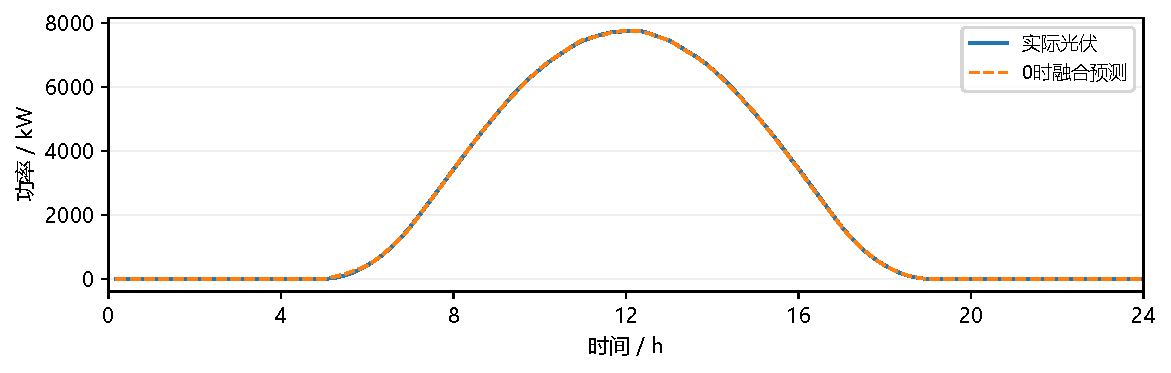
\includegraphics[width=0.86\textwidth]{figures/q3_forecast.pdf}
  \caption{光伏日前预测与实际出力的日内均值对比}
  \label{fig:q3_fc}
\end{figure}

\begin{figure}[ht]
  \centering
  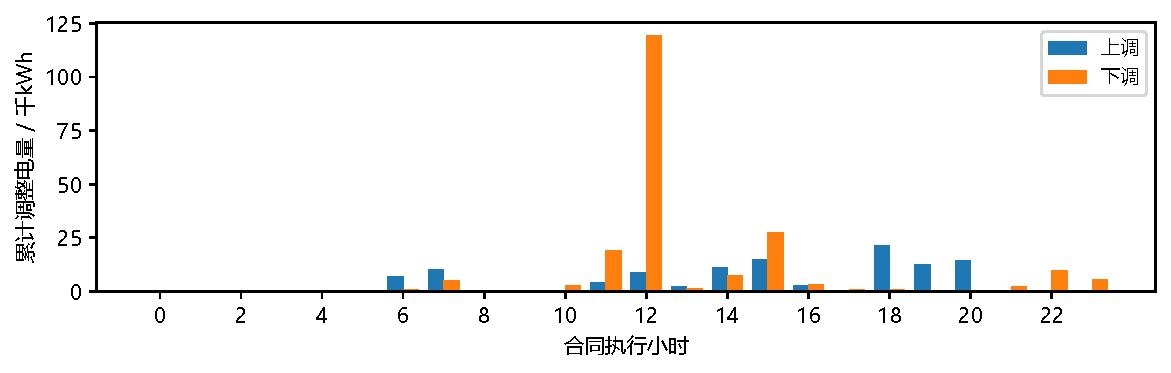
\includegraphics[width=0.86\textwidth]{figures/q3_adjust.pdf}
  \caption{各执行小时的全年上调与下调电量}
  \label{fig:q3_adj}
\end{figure}

\subsubsection{日前组合预测的时序回测}
我们采用滚动预测起点评价方法\cite{hyndman2021fpp}，以1月数据初始化误差档案，依次在2月1日至12月31日的每日0时预测随后144个时段。预测值提交后冻结，日终计算误差并更新档案。固定原模型参数重新运行预测模块，负载及融合光伏的逐时段输出均与正式轨迹一致。评价中始终用预测起点之前的观测更新估计量。

在48096个未来目标时段上，我们得到历史光伏预测与组合预测的MAE分别为150.18和127.90 kW，后者降低14.83\%；RMSE由306.25降至255.83 kW，降低16.46\%。组合预测的月度MAE范围为74.27至155.15 kW，月度误差随出力规模变化，因此同时以加权绝对百分比误差衡量相对预测精度，定义见模型检验部分。年度组合预测WAPE为5.38\%。

问题三较问题二的月度费用降幅为0.94\%至8.21\%。

\begingroup
\scriptsize
\setlength{\tabcolsep}{3pt}
\renewcommand{\arraystretch}{1.25}
\setlength{\LTpre}{6pt}
\setlength{\LTpost}{6pt}
\Needspace{0.30\textheight}
\begin{longtable}{>{\centering\arraybackslash}p{.18\textwidth}*{4}{>{\centering\arraybackslash}p{.18\textwidth}}}
\caption{问题三指定日期生效购电量（kWh）及全天购电结果}\\
\toprule 时间段 & 2025.3.20 & 2025.6.21 & 2025.9.23 & 2025.12.21\\\midrule
\endfirsthead
\caption{问题三指定日期生效购电量及全天购电结果（续）}\\
\toprule 时间段 & 2025.3.20 & 2025.6.21 & 2025.9.23 & 2025.12.21\\\midrule\endhead
10:00--10:10 & 0.00 & 0.00 & 0.00 & 0.00\\
12:00--12:10 & 535.60 & 0.00 & 467.87 & 942.55\\
14:00--14:10 & 0.00 & 0.00 & 0.00 & 0.00\\
16:00--16:10 & 531.95 & 209.95 & 570.15 & 807.99\\
18:00--18:10 & 711.82 & 0.00 & 775.78 & 734.26\\
20:00--20:10 & 0.00 & 0.00 & 0.00 & 0.00\\
全天计划量（kWh） & 63531.04 & 41438.03 & 71292.83 & 96263.52\\
全天生效量（kWh） & 63531.04 & 41438.03 & 71292.83 & 96263.52\\
全天购电费（元） & 39316.55 & 22885.89 & 44250.47 & 61769.27\\
\bottomrule
\end{longtable}
\begin{longtable}{>{\centering\arraybackslash}p{.18\textwidth}*{4}{>{\centering\arraybackslash}p{.18\textwidth}}}
\caption{问题三指定日期储能设备充放电量（kWh）}\\
\toprule 时间段 & 2025.3.20 & 2025.6.21 & 2025.9.23 & 2025.12.21\\\midrule
\endfirsthead
\caption{问题三指定日期储能设备充放电量（续，kWh）}\\
\toprule 时间段 & 2025.3.20 & 2025.6.21 & 2025.9.23 & 2025.12.21\\\midrule\endhead
0:00--4:00 & 1570.91/232.37 & 673.68/186.31 & 2403.00/26.46 & 2224.62/209.76\\
4:00--8:00 & 795.34/5903.45 & 540.32/1814.42 & 126.66/5987.36 & 1362.13/1567.22\\
8:00--12:00 & 5849.49/2777.38 & 9258.81/0.00 & 6104.69/1896.62 & 5514.79/7358.93\\
12:00--16:00 & 5058.52/291.67 & 0.00/0.00 & 3991.51/520.55 & 7437.43/2299.03\\
16:00--20:00 & 98.75/5637.82 & 69.19/5674.10 & 226.48/5574.21 & 24.06/5704.02\\
20:00--24:00 & 4164.97/2997.46 & 8711.92/2531.66 & 8526.89/3001.31 & 8498.67/2842.53\\
0时/24时储电 & 9039.75/5001.54 & 3597.51/9585.48 & 8666.71/9011.90 & 8620.43/8974.30\\
\bottomrule
\end{longtable}
\begin{longtable}{>{\centering\arraybackslash}p{.24\textwidth}p{.40\textwidth}p{.20\textwidth}}
\caption{问题三指定日期紧急购电结果（kWh）}\\
\toprule 日期 & 紧急购电时间段 & 购电量\\\midrule
\endfirsthead
\caption{问题三指定日期紧急购电结果（续，kWh）}\\
\toprule 日期 & 紧急购电时间段 & 购电量\\\midrule\endhead
2025.3.20 & 无 & 0.00\\
2025.6.21 & 无 & 0.00\\
2025.9.23 & 20:20--20:30 & 6.38\\
2025.12.21 & 07:50--08:00 & 33.05\\
\bottomrule
\end{longtable}
\endgroup

